% 15. Составьте функциональную схему и опишите функциональные связи между подсистемами в составе системы, а также между подсистемами и внешней средой, которые Вы предполагаете учитывать при разработке математической модели системы.
% 16. Какую систему (или системы) Вы готовы рассматривать как актуальный прототип по отношению к системе, рассматриваемой в Вашей работе?
% 17. Какую задачу – анализа или синтеза системы – Вы решаете? Как решаемая задача связана с целью Вашего исследования?
% 18. Укажите тип математической модели (аналитическая, основанная на использовании физических законов и/или теории, имитационная, эмпирическая), которую Вы будете использовать для решения задачи анализа системы.
% 19. Охарактеризуйте кратко особенности разрабатываемой Вами модели системы.
% 20. В каком состоянии находится разработка модели в настоящее время?
% 21. В какой среде программирования Вы реализуете модель системы?
% 22. Если в работе решается задача синтеза системы, то какой алгоритм оптимизации альтернативы системы Вы используете или предполагаете использовать?
% 23. Если при синтезе системы рассматриваются несколько показателей ее эффективности, то как решается задача оптимизации системы по векторному критерию?

Попытки описания механизмов, позволяющих реализовать разделение функционала уже существуют в наше время. Примером является Equenox - реализация спецификации OSGI, которая лежит в основе IDE Eclipse.

Спецификация OSGI предполагает построение (синтез) системы из обособленных компонентов. Для разделения зависимостей на сторонние библиотеки и сервисы. Степень разделения и ее характер зависит от реализации. В IDE Eclipse она реализована для решения целей и задач стоящих перед самой IDE, однако предполагает ее расширение по правилам конкретного бизнеса.

В рамках диссертационного иссследования, следуя правилам спецификации OSGI, мною на языке программирования Java написано решение подзадачи изменения исходного графа с учетом разрешения циклических зависимостей между файлами исходного кода. В решении получены результаты экспериментов для оценки времени работы приложения от типа используемых коллекций, в которых хранится информация о графе:
\begin{enumerate}
    \item вершины - файлы исходного кода и требования к ПО;
    \item ребра - зависимости между файлами исходного кода и трассируемость требований к ПО.
\end{enumerate}

Работа алгоритма заключается в итеративном поиске циклов в графе с последующим слиянием входящем в цикл вершин до тех пор, пока в графе не будут отсутствовать циклы.

Схема разработанного решения приведена на рисунке \ref{fig:application_scheme}.

\begin{figure}[H]
    \centering
    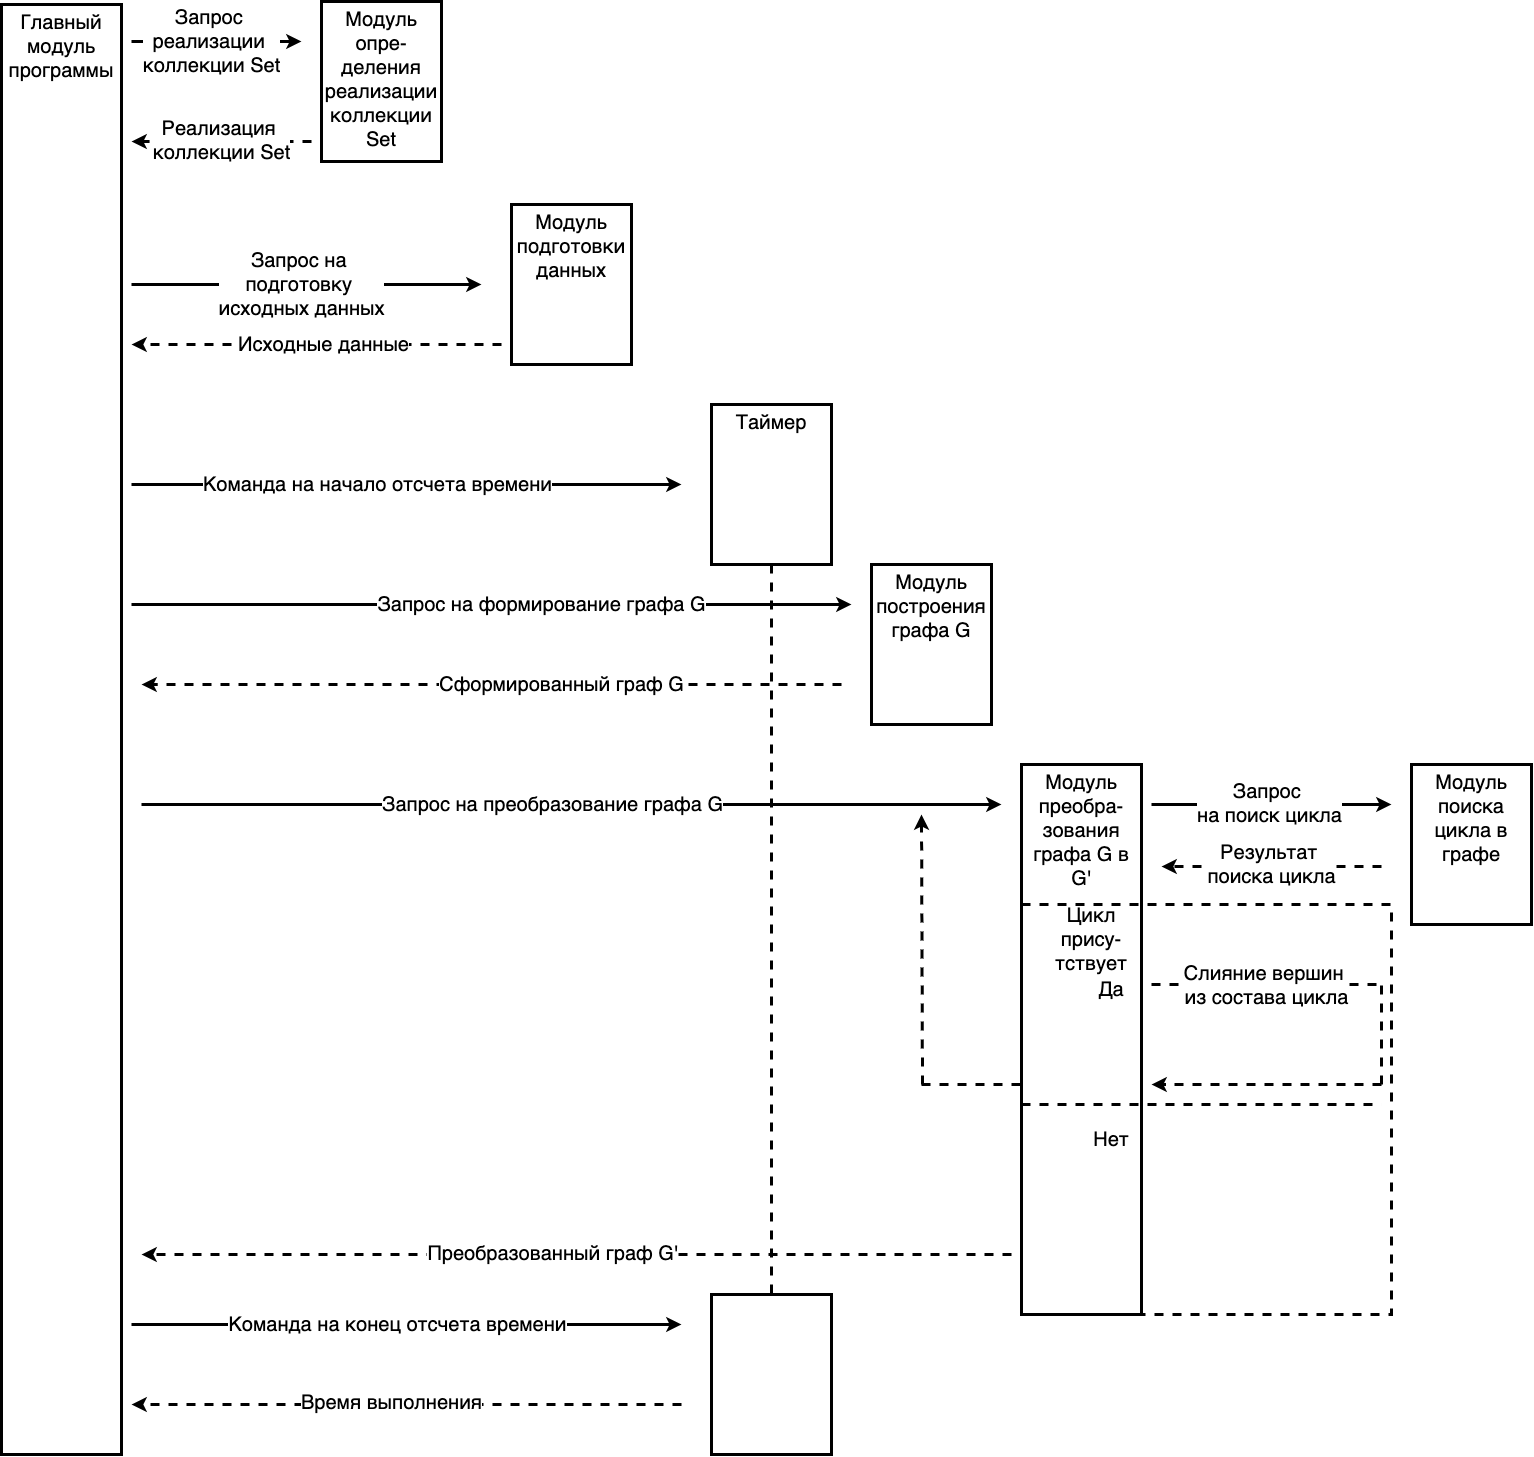
\includegraphics[width=1\textwidth]{application_scheme}
    \caption{Схема разработанного решения}
    \label{fig:application_scheme}
\end{figure}

В дальнейшем предполагается доработка модели для поиска оптимального распределения файлов исходного кода по плагинам.

Для выявления лучшего решения сформулирован векторный критерий:
\begin{enumerate}
    \item возможность динамеческого ценнобразования поставки $C_{d}$;
    \item $V_{c}$;
    \item $K_{f}$;
\end{enumerate}

% Рассказать про каждый коэффициент, какой диапазон значений принимает
$C_{d}$ является определяющим фактором. Именно благодара ему достигается динамическое изменение $K_{f}$ при статических $R^{*}$ и $V_{c}$.

$ C_{d} =
  \begin{cases}
    1 & \quad \text{если } \{ R^{'} | R^*_{d} \} \quad \exists R^{'} \in R^{*}_{un}\\
    0 & \quad \text{если } \{ R^{'} | R^*_{d} \} \quad \not \exists R^{'} \in R^{*}_{un}
  \end{cases}
$

$V_{c}$ определяет общий объем кодовой базы, поддержку которого необходимо осуществлять. Чем больше объем, тем более дорогой является поддержка.

$ V_{c} =
  \begin{cases}
    1 & \quad \text{если } N_{p} = 1 \\
    2 & \quad \text{если } 1 < N_{p} < N_{f} \\
    3 & \quad \text{если } N_{p} = N_{f}
  \end{cases}
$

$K_{f}$ не статичен и может быть уникален для каждой из поставок.

Так, вектора показателей эффективности для сформулированных альтернати в предлагаемого решения следующие:
\begin{enumerate}
    \item альтернатива по схеме <<1 требование - 1 файл исходного кода - 1 плагин>>:
    \begin{itemize}
        \item $C_{d} = 1$;
        \item $V_{c} = 3$;
        \item $K_{f} = 0$.
    \end{itemize}
    \item альтернатива по схеме <<все требования - 1 плагин>>:
    \begin{itemize}
        \item $C_{d} = 0$;
        \item $V_{c} = 1$;
        \item $K_{f} \approx 1$.
    \end{itemize}
    \item предлагаемое решение:
    \begin{itemize}
        \item $C_{d} = 1$;
        \item $V_{c} = 2$;
        \item $0 < K_{f} < 1$.
    \end{itemize}
\end{enumerate}

В предлагаемом решении $C_{d}$ = 1, что обеспечивает главное условие - динамическое изменение $K_{f}$ при статических $R^{*}$ и $V_{c}$. Несмотря на увеличение $V_{c}$ по сравнению со схемой <<все требования - 1 плагин>>, $V_{c}$ не увеличивается на столько как в схеме <<1 требование - 1 файл исходного кода - 1 плагин>>. Применяя различные алгоритмы оптимизации, приследуется цель выявления такой декомпозиции, которая обеспечивала бы минимизацию значения $K_{f}$. Предполагается использовать следующие алгоритмы оптимизации:
\begin{enumerate}
    \item генетический алгоритм;
    \item PageRank;
    \item решающий лес.
\end{enumerate}